%%%%%%%%%%%%%%%%%%%%%%%%%%%%%%%%%%%%%%%%%%%%%%%%%%%%%%%%%%%%%%%%%%%%%%%%%%%%%%%%%%%%%%%%%%%
%% Ultimas modificacoes, 06/02/2012 - Alexandre Duarte 
%% Baseado no modelo latex de Isaac Maia (COPIN/UFCG)
%%
%% Para utilizar ese modelo sao necessarios os seguintes arquivos:
%%
%% ppgi.cls
%% ppgi.sty
%% mestre.sty
%%
%%
%% Mais detalhes sobre normas ABNT no latex, consultar http://abntex.codigolivre.org.br
%% Wiki interessante com dicas uteis sobre latex : http://www.tex-br.org
%%
%%
%% Para compilar esse arquivo, e' sempre importante fazer duas passagens com latex
%%%%
%%%%%%%%%%%%%%%%%%%%%%%%%%%%%%%%%%%%%%%%%%%%%%%%%%%%%%%%%%%%%%%%%%%%%%%%%%%%%%%%%%%%%%%%%%%

\documentclass[a4paper,titlepage]{ppgi}\usepackage[]{graphicx}\usepackage[]{color}
%% maxwidth is the original width if it is less than linewidth
%% otherwise use linewidth (to make sure the graphics do not exceed the margin)
\makeatletter
\def\maxwidth{ %
  \ifdim\Gin@nat@width>\linewidth
    \linewidth
  \else
    \Gin@nat@width
  \fi
}
\makeatother

\definecolor{fgcolor}{rgb}{0.345, 0.345, 0.345}
\newcommand{\hlnum}[1]{\textcolor[rgb]{0.686,0.059,0.569}{#1}}%
\newcommand{\hlstr}[1]{\textcolor[rgb]{0.192,0.494,0.8}{#1}}%
\newcommand{\hlcom}[1]{\textcolor[rgb]{0.678,0.584,0.686}{\textit{#1}}}%
\newcommand{\hlopt}[1]{\textcolor[rgb]{0,0,0}{#1}}%
\newcommand{\hlstd}[1]{\textcolor[rgb]{0.345,0.345,0.345}{#1}}%
\newcommand{\hlkwa}[1]{\textcolor[rgb]{0.161,0.373,0.58}{\textbf{#1}}}%
\newcommand{\hlkwb}[1]{\textcolor[rgb]{0.69,0.353,0.396}{#1}}%
\newcommand{\hlkwc}[1]{\textcolor[rgb]{0.333,0.667,0.333}{#1}}%
\newcommand{\hlkwd}[1]{\textcolor[rgb]{0.737,0.353,0.396}{\textbf{#1}}}%

\usepackage{framed}
\makeatletter
\newenvironment{kframe}{%
 \def\at@end@of@kframe{}%
 \ifinner\ifhmode%
  \def\at@end@of@kframe{\end{minipage}}%
  \begin{minipage}{\columnwidth}%
 \fi\fi%
 \def\FrameCommand##1{\hskip\@totalleftmargin \hskip-\fboxsep
 \colorbox{shadecolor}{##1}\hskip-\fboxsep
     % There is no \\@totalrightmargin, so:
     \hskip-\linewidth \hskip-\@totalleftmargin \hskip\columnwidth}%
 \MakeFramed {\advance\hsize-\width
   \@totalleftmargin\z@ \linewidth\hsize
   \@setminipage}}%
 {\par\unskip\endMakeFramed%
 \at@end@of@kframe}
\makeatother

\definecolor{shadecolor}{rgb}{.97, .97, .97}
\definecolor{messagecolor}{rgb}{0, 0, 0}
\definecolor{warningcolor}{rgb}{1, 0, 1}
\definecolor{errorcolor}{rgb}{1, 0, 0}
\newenvironment{knitrout}{}{} % an empty environment to be redefined in TeX

\usepackage{amsmath}
\usepackage{alltt}
\usepackage[portuguese,ruled,linesnumbered]{algorithm2e}
\usepackage[english,portuges]{babel}
\usepackage{ppgi,mestre,epsfig}
\usepackage{times}
\usepackage[final]{pdfpages}
\usepackage{hyperref}
\hypersetup{
    bookmarks=true,   
    pdftitle={Monitor legislativo},
    pdfauthor={Vitor Márcio Paiva de Sousa Baptista}, 
    pdfsubject={Modelo de Documento Científico},
    pdfkeywords={Dissertação, Mestrado, PPGI, UFPB, modelo}, 
    colorlinks=true,
    linkcolor=black,
    citecolor=black,
    filecolor=black,
    urlcolor=black
 }

% Corrige bug no algorithm2e que usa termos em espanhol ao invés de português
\SetKwFor{Para}{para}{fa\c{c}a}{fim para}
\SetKwFor{ParaPar}{para}{fa\c{c}a em paralelo}{fim para}
\SetKwFor{ParaCada}{para cada}{fa\c{c}a}{fim para cada}
\SetKwFor{ParaTodo}{para todo}{fa\c{c}a}{fim para todo}

%-------------------------- Para usar acentuacaoo em sistemas ISO8859-1 ------------------------------------
% Se estiver usando o Microsoft Windows ou linux com essa codificacao, descomente essas linhas abaixo
% e comente as linhas referentes ao UTF8
%\usepackage[applemac]{inputenc} % Usar acentuacao em sistemas ISO8859-1, comentar a linha com  \usepackage[utf8x {inputenc}
%-----------------------------------------------------------------------------------------------------

%-------------------------- Para usar acentuacao em sistemas UTF8 ------------------------------------
% Para a maior parte das distribuicoes linux, usar essa opcao
\usepackage{ucs}
\usepackage[utf8x]{inputenc}
\usepackage[T1]{fontenc}
%-----------------------------------------------------------------------------------------------------
\usepackage{float}      
\usepackage{fancyvrb}
\usepackage{fancyheadings}
\usepackage{tikz} % Permite usar math mode dentro dos gráficos do knitr
\usepackage{graphicx}
\graphicspath{{figure/}}
\setkeys{Gin}{width=0.5\textwidth}
\usepackage{longtable} %tabelas longas, para tabelas que ultrapassam uma pagina
\usepackage{pdflscape} % landscape figures
\usepackage{glossaries} % Gerar glossário
\usepackage[skip=0pt]{caption} % Diminui distância entre imagens/tabelas e seus captions
\usepackage{subcaption}
\newcommand{\subfloat}[2][need a sub-caption]{\subcaptionbox{#1}{#2}}

\makeglossaries
\newacronym{IR}{IR}{Índice de Rice}
\newacronym{PT}{PT}{Partido dos Trabalhadores}
\newacronym{PSOL}{PSOL}{Partido Socialismo e Liberdade}
\newacronym{API}{API}{\emph{Application Programming Interface}}
\newacronym{XML}{XML}{\emph{eXtensible Markup Language}}
\newacronym{CSV}{CSV}{\emph{Comma Separated Values}}
\newacronym{JSON}{JSON}{\emph{JavaScript Object Notation}}
\newacronym{CEBRAP}{CEBRAP}{Centro Brasileiro de An\'alise e Pesquisa}

%\input{psfig.sty}
% ----------------- Para inserir codigo fonte de linguagens de programacao no documento -------------
\usepackage{listings}
\lstset{numbers=left,
stepnumber=1,
firstnumber=1,
numberstyle=\scriptsize,
extendedchars=true,
breaklines=true,
frame=tb,
basicstyle=\scriptsize,
stringstyle=\ttfamily,
showstringspaces=false
}
\renewcommand{\lstlistingname}{C\'odigo Fonte}
\renewcommand{\lstlistlistingname}{Lista de C\'odigos Fonte}

% ---------------------------------------------------------------------------------------------------

\selectlanguage{portuges}
\sloppy

\setcounter{secnumdepth}{4}
\setcounter{tocdepth}{4}
\usepackage{abnt-alf}

% Centraliza todos os floats
\makeatletter
\g@addto@macro\@floatboxreset\centering
\makeatother
\IfFileExists{upquote.sty}{\usepackage{upquote}}{}
\begin{document}


%%%%%%%%%%%%%%%%%%%%%%%%%%%%%%%%%%%%%%%%%%%%%%%%%%%%%%%%%%%%%%%%%%%%%%%%%%%%%%%%
\Titulo{Um modelo para a previsão da entrada ou saída\\da coalizão pelos deputados federais}
\Autor{Vitor Márcio Paiva de Sousa Baptista}
\Data{06 de Março de 2012}
\Area{Ciência da Computação}
\Pesquisa{Computação Distribuída | Sinais, Sistemas Digitais e Gráficos}
\Orientadores{Alexandre Nóbrega Duarte\\ (Orientador)}

\newpage
\cleardoublepage
\PaginadeRosto

\newpage
\cleardoublepage

%%%%%%%%%%%%%%%%%%%%%%%%%%%%%%%%%%%%%%%%%%%%%%%%%%%%%%%%%%%%%%%%%%%%%%%%%%%%%%%%
\begin{resumo} 
Vestibulum varius accumsan odio malesuada gravida. Duis a erat et arcu tincidunt semper sed et quam. Sed mattis semper quam vel imperdiet. Etiam tortor orci, ullamcorper ac aliquam eu, interdum quis justo. Morbi lacinia ligula ac nibh imperdiet semper. Aliquam varius tristique nisl, in blandit tellus ultrices et. Nullam est nisl, pretium sit amet vehicula quis, cursus at enim.
\\
\\
\textbf{Palavras-chave:} Palavras, chave, para, seu, trabalho.

\end{resumo}
%\newpage
%\cleardoublepage

%%%%%%%%%%%%%%%%%%%%%%%%%%%%%%%%%%%%%%%%%%%%%%%%%%%%%%%%%%%%%%%%%%%%%%%%%%%%%%%%
\begin{summary}
In Brazil, there are tools for monitoring the behaviour of legislators in
rollcalls, such as O Estado de São Paulo's Basômetro and Radar Parlamentar.
These tools are used both by journalists and political scientists for analysis.

Although they are great analysis tools, their usefulness for monitoring is
limited because they require a manual follow-up, which makes it a lot of work
when we consider the volume of data. Only in the Chamber of Deputies, 513
legislators participate on average over than 400 rollcalls by legislature. It
is possible to decrease the amount of data analyzing the parties as a whole,
but in contrast we lose the ability to detect individuals' drives or
intra-party groups such as factions.

In order to mitigate this problem, I developed a statistical model that detects
when a legislator changes his or her position, joining or leaving the
governmental coalition, through ideal points estimates using the W-NOMINATE. It
can be used individually or integrated to tools such as Basômetro, providing a
filter for researchers find the deputies who changed their behaviour most
significantly.

The universe of study is composed of legislators from the Chamber of Deputies
from the 50th to the 54th legislatures, starting in the first term of Fernando
Henrique Cardoso in 1995 until the end of the first term of Dilma Rousseff in
2015.

\textbf{Keywords:} Legislative Analysis, Political Science, Data Science,
Predictive Models, Machine Learning.

\end{summary}

%\newpage
%\cleardoublepage

%%%%%%%%%%%%%%%%%%%%%%%%%%%%%%%%%%%%%%%%%%%%%%%%%%%%%%%%%%%%%%%%%%%%%%%%%%%%%%%%
% TMP: Agradecimentos
\begin{agradecimentos}
Donec ultricies elit a quam ornare posuere. Pellentesque eu tortor massa. Aliquam erat volutpat. In vitae justo dolor, ac fringilla nisl. In hac habitasse platea dictumst. Pellentesque placerat eleifend sem, in tempor nisl elementum fermentum. Ut in metus vitae magna volutpat viverra. Suspendisse ac dolor velit, in volutpat magna. Cras blandit urna quis diam feugiat volutpat. Nunc mattis lobortis libero varius posuere. Integer sem augue, aliquet fringilla porta nec, adipiscing sed ante. Aenean feugiat, eros non vehicula pretium, neque purus vehicula diam, eu vulputate leo neque nec velit. Vestibulum at orci quam, et mattis tortor. Donec iaculis orci enim.

\end{agradecimentos}

\clearpage

%%%%%%%%%%%%%%%%%%%%%%%%%%%%%%%%%%%%%%%%%%%%%%%%%%%%%%%%%%%%%%%%%%%%%%%%%%%%%%%%
%% Definicao do cabecalho: secao do lado esquerdo e numero da pagina do lado direito
\pagestyle{fancy}
\addtolength{\headwidth}{\marginparsep}\addtolength{\headwidth}{\marginparwidth}\headwidth = \textwidth
\renewcommand{\chaptermark}[1]{\markboth{#1}{}}
\renewcommand{\sectionmark}[1]{\markright{\thesection\ #1}}\lhead[\fancyplain{}{\bfseries\thepage}]%
	     {\fancyplain{}{\emph{\rightmark}}}\rhead[\fancyplain{}{\bfseries\leftmark}]%
             {\fancyplain{}{\bfseries\thepage}}\cfoot{}

%%%%%%%%%%%%%%%%%%%%%%%%%%%%%%%%%%%%%%%%%%%%%%%%%%%%%%%%%%%%%%%%%%%%%%%%%%%%%%%%

\Sumario
\ListadeSiglas
\listoffigures
\listoftables
\lstlistoflistings %lista de codigos fonte - Para inserir a listagem de
% codigos fonte

\newpage
\cleardoublepage
\Introducao


%%%%%%%%%%%%%%%%%%%%%%%%%%%%%%%%%%%%%%%%%%%%%%%%%%%%%%%%%%%%%%%%%%%%%%%%%%%%%%%%
%
% Hifenizacao - Colocar lista de palavras que nao devem ser separadas e que 
% nao estao no dicionario portuges.
% As palavras do dicionario portuges ja sao separadas corretamente pelo lateX
%
\hyphenation{ gLite OurGrid GridDoctor }

%%%%%%%%%%%%%%%%%%%%%%%%%%%%%%%%%%%%%%%%%%%%%%%%%%%%%%%%%%%%%%%%%%%%%%%%%%%%%%%%
%% A partir daqui coloque seus capitulos. Sugere-se que eles sejam inseridos com o comando \input
%% Da seguinte maneira:
%% 



\chapter{Introdução} \label{intro}

\section{Motivação}\label{sec:motiva}

A quantidade de dados relacionados a atividade dos parlamentares brasileiros é muito grande. Exemplos simples são as votações, presenças em plenário, projetos de Lei, viagens, candidaturas, etc. Analisar manualmente esse volume de dados é uma tarefa bastante difícil e por isso podem haver situações importantes que não sejam percebidas. Visando auxiliar no processo de acompanhamento e fiscalização da atividade dos parlamentares brasileiros este trabalho propõe uma ferramenta de monitoramento automático e contínuo que gera alertas e relatórios sobre o que acontece nas casas legislativas brasileiras, usando a Câmara dos Deputados como estudo de caso.

\section{Objetivos}

O objetivo geral desta dissertação é o desenvolvimento e validação de um modelo
capaz de prever quando um deputado federal irá deixar ou entrar na coalizão do
governo a partir das votações nominais.

\subsection{Objetivos Especificos}

\begin{itemize}
\item Desenvolver um mecanismo capaz de detectar mudanças no padrão de comportamento dos parlamentares;
\item Desenvolver um mecanismo capaz de detectar mudanças semelhantes entre grupos de parlamentares (ex.: João e Pedro sempre divergiram em seus votos e de repente passaram a concordar);
\item Desenvolver um mecanismo capaz de detectar votações importantes/polêmicas (falta definir o que são importante e polêmica)
\end{itemize}

\section{Metodologia}

Não sei qual o nome da metodologia que estou usando: por enquanto é tudo muito ad-hoc. Estudo de caso é um componente, mas não sei se há outra.

Alexandre -  Não é preciso dar uma nome a metodologia. O que você precisa descrever aqui são os passos seguidos até chegar ao resultado final.

Tipo
1 - Levantamento Bibliográfico sobre X e Y
2 - Desenvolviment do mecanismo para extração e filtragem dos dados
3 - ...

\section{Publicações Relacionadas}

Mencionar o artigo que você publicou no BRASNAM

\section{Estrutura da Dissertação}

Descrever a estrutura dos demais capítulos. Melhor fazer isso só no final.


\chapter{Fundamentação Teórica}\label{cap:fundamentacao}

\section{Ciência de Dados}

Segundo \citeonline{Stanton2012}, o termo Ciência de Dados (do inglês
\emph{Data Science}) é usado para definir uma área emergente que se ocupa da
coleta, preparo, análise, visualização, gestão e preservação de conjuntos de
dados com o objetivo de extrair conhecimento. Ela usa a ciência da computação
como ferramenta para extrair modelos estatísticos a partir de dados relativos a
uma área fim, como a ciência política.

Por ser uma área interdisciplinar e relativamente recente (especialmente no
Brasil) a distinção do que é ciência de dados e não estatística, matemática ou
computação pode ainda não ser muito clara \cite{Porto2014}. Para facilitar essa
diferenciação, \citeonline{Conway2013} criou o diagrama de Venn da figura
\ref{fig:ciencia-de-dados-venn} que mostra onde está a ciência de dados em
relação as outras áreas.

\begin{figure}[h]
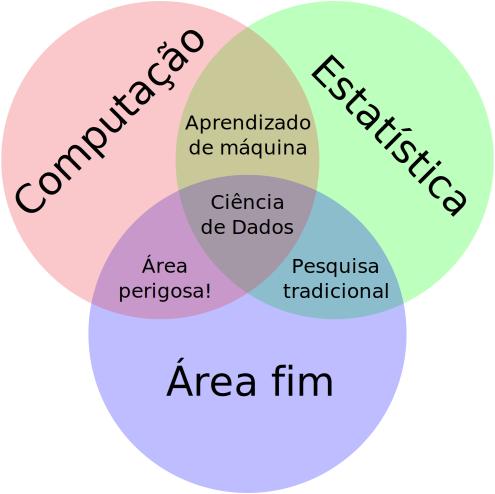
\includegraphics{ciencia-de-dados-diagrama-venn}
\caption{Diagrama de Venn mostrando as habilidades necessárias para um
cientista de dados}
\label{fig:ciencia-de-dados-venn}
\end{figure}

Com as técnicas da ciência de dados, podemos responder perguntas como ``Qual a
melhor rota para chegar até meu trabalho?'', ``Vai chover hoje?'', ``Quais são
minhas chances de desenvolver câncer nos próximos 10 anos?''. Neste trabalho,
estamos interessados nas técnicas de desenvolvimento de modelos preditivos que,
baseados nos dados e conhecimento que temos do assunto, determinam a
probabilidade de acontecimentos futuros.

\subsection{Modelos preditivos}

\citeonline{Geisser1993} define modelagem preditiva como sendo ``o processo
pelo qual um modelo é criado ou escolhido para tentar melhor prever a
probabilidade de um resultado''. Já \citeonline{Kuhn2013} definem como ``o
processo de desenvolvimento de uma ferramenta ou modelo matemático que gere uma
previsão precisa''.

Independente da definição usada, modelos preditivos fazem parte do dia-a-dia da
sociedade atual. O Google os utiliza para interpretar o que seus usuários estão
buscando; o Netflix usa para recomendar filmes; corretoras de valores usam para
definir que ações comprar ou vender; seguradoras usam para definir qual o risco
e, consequentemente, o preço do seguro de um carro, entre outros
\cite{Levy2010}.

Existem duas principais categorias de problemas que podem ser resolvidos por
modelos preditivos: regressão e classificação. A diferença entre eles está no
tipo de resposta que queremos prever, se é contínua ou categórica, que
influencia nos tipos de modelos que podem ser usados e na forma de avaliá-los.
Por exemplo, ao analisarmos modelos que preveem o preço de um imóvel a partir
da sua área, buscamos o que chegue mais próximo do valor real\footnote{Esta é
uma simplificação. Existem diversas outras características a serem analisados
ao escolher um modelo, como facilidade de interpretação, velocidade de
execução, entre outras. Aqui consideramos que a única diferença entre eles seja
o resultado previsto.}. Já ao avaliar modelos que classifiquem imagens dos
dígitos 0 a 9, só nos interessamos na classificação correta; dois modelos que
identifiquem a imagem do número 1 como sendo do número 3 e 8 estão igualmente
errados. O que classificou como 3 não está ``menos errado'' do que o que
classificou como 8 \cite{Kuhn2013,Zumel2014}. Neste trabalho, nosso foco é em
classificação.

\subsection{Avaliando performance em modelos de classificação}

O primeiro passo para melhorar algo é conseguir mensurá-lo, ao contrário não
saberemos se nossas modificações estão melhorando ou piorando a situação. Com
relação a modelos preditivos, o ideal é ter uma métrica única que defina sua
performance de acordo com nossos critérios. Dessa forma, a comparação e
otimização dos modelos é simplificada \cite{Ng2012}.

Uma das formas mais comuns de descrever a perfomance de um modelo de
classificação é através de uma ``matriz de confusão''. A tabela
\ref{table:exemplo-matriz-de-confusao} mostra um exemplo de matriz de confusão
com duas categorias: ``positivo'' e ``negativo''. Na diagonal principal estão
os valores classificados corretamente, e fora dela estão os erros. Dessa matriz
podemos extrair diversas métricas, como:

\begin{table}
\centering
\begin{tabular}{c c c}
  Previsto & \multicolumn{2}{c}{Observado} \\  \cline{2-3}
  & \multicolumn{1}{|c}{Positivo} & \multicolumn{1}{c|}{Negativo} \\
  \hline
  \multicolumn{1}{|c|}{Positivo} & Verdadeiro positivo (VP) & \multicolumn{1}{c|}{Falso positivo (FP)} \\
  \multicolumn{1}{|c|}{Negativo} & Falso negativo (FN) & \multicolumn{1}{c|}{Verdadeiro negativo (VN)} \\
  \hline
\end{tabular}
\caption{Matriz de confusão para um problema com duas classes: ``positivo'' e
``negativo''.}
\label{table:exemplo-matriz-de-confusao}
\end{table}

\begin{description}
\item[Número de amostras positivas]
\begin{equation}
\label{eq:positive-rate}
P = VP + FN
\end{equation}
\item[Número de amostras negativas]
\begin{equation}
\label{eq:negative-rate}
N = VN + FP
\end{equation}
\item[Acurácia] Proporção de predições corretas
\begin{equation}
\label{eq:accuracy}
ACC = \frac{VP + VN}{P + N}
\end{equation}
\item[Sensibilidade] Proporção de elementos da classe positiva classificados
corretamente com relação ao total de elementos positivos
\begin{equation}
\label{eq:sensitivity}
SENS = \frac{VP}{VP + FN}
\end{equation}
\item[Especificidade] Proporção de elementos da classe negativa classificados
corretamente com relação ao total de elementos negativos
\begin{equation}
\label{eq:specificity}
ESPEC = \frac{VN}{FP + VN}
\end{equation}
\end{description}

Dessas métricas, a com interpretação mais simples é a acurácia (equação
\ref{eq:accuracy}), que mede o percentual de predições corretas. Entretanto,
ela tem algumas limitações. Primeiramente, ela não leva em consideração o tipo
do erro. Em diversos problemas, o custo de um falso positivo é diferente do de
um falso negativo. Por exemplo, num sistema de classificação de spam, é
preferível que o usuário veja uma propaganda (falso negativo) do que deixe de
receber um e-mail importante (falso positivo). Além disso, ela também não
considera a frequência natural de cada classe. Se, por exemplo, 90\% dos
e-mails que eu receba não sejam spam, um modelo que simplesmente classifique
todo e-mail como não sendo spam terá 90\% de acurácia \cite{Kuhn2013}.

O \emph{Kappa} é uma métrica que leva em consideração as proporções das
classes. Ela pode assumir valores entre -1 e 1, sendo que 1 indica que todas as
predições foram corretas, -1 indica que todas foram erradas, e 0 que o modelo
tem uma performance igual a um modelo aleatório. A equação \ref{eq:kappa}
mostra como calculá-la, onde $ACC$ é a acurácia observada e $ACC_{esperada}$ é
a acurácia esperada \cite{Cohen1960}.

\begin{equation}
\label{eq:kappa}
Kappa = \frac{ACC - ACC_{esperada}}{1 - ACC_{esperada}}
\end{equation}

Em geral, o resultado do uso de modelos de classificação é a probabilidade de
pertencimento a cada categoria. Por exemplo, um modelo pode, ao analisar um
e-mail, determinar que ele tem 75\% de chances de ser spam e, consequentemente,
25\% de chances de não ser. Para transformar essa probabilidade em uma
categoria, define-se um ponto de corte. Por padrão, ele é definido em grande
parte das ferramentas como 50\%. Usando esse valor, o exemplo anterior seria
classificado como spam \cite{Kuhn2013}.

Esse padrão é uma escolha interessante caso o custo de um falso positivo ou
falso negativo seja o mesmo e as categorias sejam balanceadas. Caso contrário,
é recomendável testar outros valores. Uma ferramenta para analisar a
sensibilidade e especificidade de um modelo usando diferentes pontos de corte é
a curva ROC (\emph{Receiver Operator Characteristic}). Essa visualização mostra
os valores de sensibilidade e especificidade em diferentes pontos de corte
\cite{Altman1994,Brown2006,Fawcett2006}.

A figura \ref{fig:exemplo-roc} mostra um exemplo de uma curva ROC com os
valores discriminados em dois pontos. A partir desse gráfico, percebemos a
troca entre sensibilidade e especificidade (quanto maior um, menor o outro), e
podemos escolher o melhor ponto de corte para o modelo em questão levando em
consideração nossos objetivos.

\begin{knitrout}
\definecolor{shadecolor}{rgb}{0.969, 0.969, 0.969}\color{fgcolor}\begin{figure}
\includegraphics[width=\maxwidth]{figure/tmp/exemplo-roc-1} \caption[Curva ROC de um modelo mostrando a área sob a curva (AUC) e dois pontos de corte]{Curva ROC de um modelo mostrando a área sob a curva (AUC) e dois pontos de corte: 0,5, o mais comum, e 0,614, o mais próximo do canto superior esquerdo.}\label{fig:exemplo-roc}
\end{figure}


\end{knitrout}

Além de auxiliar na escolha do ponto de corte, a curva ROC também pode ser
usada para avaliar e comparar modelos desenhando-os num mesmo gráfico ou
comparando a área sob suas curvas (AUC). O modelo na figura
\ref{fig:exemplo-roc} possui AUC 0,787. Quanto mais próximo a curva está do
canto superior esquerdo, maior é seu AUC e, consequentemente, maior é sua
performance. O modelo perfeito tem AUC 1, já um modelo aleatório tem AUC
próximo de 0,5 e segue na diagonal do gráfico. O que caracteriza é um AUC bom
ou ruim varia de caso a caso, mas \citeonline{HosmerJr2013} definiram uma regra
geral para avaliação descrita na tabela \ref{table:valores-auc}.

\begin{table}
\centering
\begin{tabular}{c l}
  AUC & \multicolumn{1}{c}{Valor} \\
  \hline
  0,5 & Não há discriminação \\
  Entre 0,7 e 0,8 & Discriminação aceitável \\
  Entre 0,8 e 0,9 & Discriminação excelente \\
  Acima de 0,9 & Discriminação excepcional \\
\end{tabular}
\caption{Regra geral para avaliação da área sob a curva ROC de \citeonline{HosmerJr2013}.}
\label{table:valores-auc}
\end{table}

% TODO: Concluir

% % Treinamento de algoritmos
% % Regressão VS Classificação

% Random Forest
% % Árvores de decisão

% Validação cruzada

\section{Modelos espaciais de votação}



A ideia básica de modelos espaciais de votação é que o conjunto de alternativas
políticas de uma votação pode ser tratado como uma dimensão em um espaço
euclidiano, e cada parlamentar tem preferências de valores nessa dimensão. O
voto seria então definido pela escolha da alternativa mais próxima da sua
preferência.

Há diversos modelos para estimar esses valores, como o NOMINATE, W-NOMINATE,
DW-NOMINATE, que são paramétricos; o Optimal Classification, que é
não-paramétrico, e; modelos baseados em estatística Bayesiana, como o IDEAL.
Nosso foco neste trabalho é no W-NOMINATE.
\cite{Poole2000,Poole2005,Poole2014,Jackman2000,Clinton2004}

Considere um exemplo onde 5 parlamentares votam em
dois projetos de Lei: um propondo a redução da maioridade penal de
18 para 16 anos e outra
propondo o aumento do salário-mínimo de R\$ 1.000 para
R\$ 1.200. Suponha que cada um tem uma única preferência
(\emph{single-peakedness}), conhecido como seu ponto ideal, e vota sinceramente
de acordo com ela. Considere também que as preferências são simétricas. Isto é,
dado duas escolhas a uma mesma distância do ponto ideal de um parlamentar, ele
será indiferente a qualquer uma delas.

Graficamente, temos a figura \ref{fig:modelo-espacial-votacao}, onde os pontos
representam as preferências dos legisladores sobre cada votação, representados
como as dimensões nesse espaço euclidiano. As linhas são chamadas linhas de
corte. Elas passam pelo ponto médio entre as duas alternativas em votação: a de
votar sim e a de votar não. Em outras palavras, se as escolhas são entre uma
maioridade penal de 16 ou
18, a linha de corte passa em $\frac{16 + 18}{2}$,
ou seja, $17$. Ela divide os legisladores que irão votar não, que estão a
esquerda da linha, dos que irão votar sim, que estão a direita da mesma. Caso
esteja sobre a linha de corte, ele é indiferente as alternativas.

\begin{knitrout}
\definecolor{shadecolor}{rgb}{0.969, 0.969, 0.969}\color{fgcolor}\begin{figure}
\includegraphics[width=\maxwidth]{figure/tmp/modelo-espacial-votacao-1} \caption[Preferências de 5 deputados em 2 votações com suas respectivas linhas de corte]{Preferências de 5 deputados em 2 votações com suas respectivas linhas de corte}\label{fig:modelo-espacial-votacao}
\end{figure}


\end{knitrout}

Nesse exemplo estamos mostrando duas dimensões, mas o algoritmo é capaz de
estimar os pontos ideais em até dez dimensões.

% FIXME: Descrever as características do W-NOMINATE e (talvez) como ele se
% diferencia dos outros.

O comportamento dos parlamentares é assumido como sendo formado por dois
componentes: um determinístico e outro estocástico. Formalmente, definimos a
utilidade do legislador $i$ na consequência política do resultado ``sim'' da
votação $j$ como sendo:

\begin{equation}
  U_{ijy} = u_{ijy} + \epsilon_{ijy}
\end{equation}

onde $u_{ijy}$ é a parte determinística e $\epsilon_{ijy}$ é a parte
estocástica da função utilidade. Se não houver erro, o legislador vota sim se
$U_{ijy} > U_{ijn}$ e não se $U_{ijy} < U_{ijn}$. Caso $U_{ijy} = U_{ijn}$, ele
é indiferente para qualquer resultado.

\begin{description}
\item[$s$] o número de dimensões indexado por $k = 1, ..., s$;
\item[$p$] o número de parlamentares indexado por $i = 1, ..., p$;
\item[$q$] o número de votações indexado por $j = 1, ..., q$;
\item[$X_i$] o ponto ideal do parlamentar $i$ em um vetor de comprimento $s$;
\item[$Z_{jy}$ e $Z_{jn}$] a representação de cada votação em um vetor de comprimento
$s$, onde $y$ e $n$ são as consequências políticas dos resultados ``Sim'' e
``Não'', respectivamente.
\end{description}

A utilidade do parlamentar $i$ para a consequência $y$ em uma votação $j$ é:

\begin{equation}
  U_{ijy} = \beta \exp^{\left( - \frac{1}{2} \sum\limits_{k=1}^s w_k^2 d_{ijky}^2 \right)}
\end{equation}

Formalmente, sendo $O_{jy}$ e $O_{jn}$ os resultados correspondendo
respectivamente a um voto ``sim'' e um voto ``não'' na votação $j$ ($j = 1,
..., q$), definimos $Z_j$ como: 

\begin{equation}\label{eq:cutpoint}
  Z_j = \frac{O_{jy} + O_{jn}}{2}
\end{equation}

O $Z_j$ pode definir um ponto, linha, plano ou hiperplano, dependendo do número
de dimensões que estamos tratando. Ele é conhecido como ponto (ou linha, etc.)
de corte.

% Introdução

%% O que são de modelos de votação?

%% Por que os modelos espaciais de votação foram criados?

%% Por que não usar os votos diretamente?

% Desenvolvimento

% Conclusão

\subsection{Comparando pontos ideais ao longo do tempo}
\label{cap:fundamentacao:comparando-pontos-ideais-no-tempo}

O principal problema em comparar mudanças nos pontos ideais ao longo do tempo é
distinguir alterações causadas por mudanças na agenda legislativa das causadas
por mudanças no posicionamento dos parlamentares \cite{Bailey2007}. Em outras
palavras, se o ponto ideal de um deputado federal passa de 0.3 para -0.2 de um ano
para o outro, como descobrir se isso representa uma mudança real de ideologia ou
é somente reflexo da diferença na agenda legislativa dos dois períodos?

Segundo \citeonline{Shor2010}, todos os esforços para resolver esse problema
usam ``pontes'', que podem ser parlamentares cujo posicionamento assume-se ter
se mantido estável durante o período de interesse, ou; projetos de Lei que
foram votados em mais de um momento (nas duas casas legislativas em um sistema
bicameral, por exemplo). O primeiro é mais usado para comparar as mudanças nos
posicionamentos dos parlamentares, enquanto o segundo permite unir pessoas que
não votaram juntas em um mesmo mapa espacial\footnote{Por exemplo,
\citeonline{Shor2010} colocam todos os legisladores de 11 estados americanos e
do congresso federal em um período que varia entre 7 e 15 anos, dependendo do
estado, em um mesmo mapa espacial}. \citeonline{Poole2005} propõe duas formas
para estimar pontos ideais usando pontes.

Na primeira, batizada de \emph{pooled scaling} por \citeonline{Shor2010},
dividimos os votos dos parlamentares que queremos mensurar em dois
parlamentares ``virtuais'', um com os votos antes e outro com os votos depois
da data de interesse. Unimos esses parlamentares virtuais com os
parlamentares-ponte, que possuem um registro único, em uma tabela individual e
executamos o algoritmo de estimação dos pontos ideais. Ao final, teremos dois
pontos para cada parlamentar de interesse e um ponto para os pontes. Na
segunda, que \citeonline{Shor2010} chamam de \emph{linear mapping}, estimamos
os pontos ideias separadamente em cada período e os conectamos usando regressão
entre os conjuntos de pontos dos parlamentares-ponte. Ambas formas devem gerar
resultados similares, mas a segunda é computacionalmente mais simples, o que
pode ser essencial, dependendo da quantidade de parlamentares e votações votos
em estudo.

\citeonline{Poole2005} ainda descreve uma terceira forma, similar a
\emph{pooled scaling} descrita acima, que usa para testar se os senadores
norte-americanos mudam de comportamento nos últimos dois anos de seus mandatos,
antes de concorrer à reeleição. Neste caso, ele quer calcular a mudança de
comportamento de todos os legisladores em dois momentos numa mesma legislatura.
Se usássemos o \emph{pooled scaling} diretamente, precisaríamos escolher alguns
parlamentares como pontes que, por definição, não teriam mudado de
comportamento. Ao invés disso, ele segue o seguinte processo:

\begin{enumerate}
  \item Para cada parlamentar, faça:
    \begin{enumerate}
      \item Transforme-o em dois parlamentares ``virtuais'', um com o conjunto
de votos antes, e outro com os depois da data de interesse. Os outros
parlamentares não são modificados;
      \item Calcule os pontos ideias;
      \item Guarde os resultados dos dois parlamentares ``virtuais''. A
diferença entre suas posições representa a mudança de comportamento do
parlamentar.
    \end{enumerate}
  \item Calcule medidas de incerteza para as estimativas.
\end{enumerate}

Ao final, ele tem dois pontos para cada senador: um representando sua posição
nos primeiros 4, e o outro nos últimos 2 anos da legislatura. Note que, como as
matrizes de votações usadas para gerar os mapas espaciais são diferentes, eles
não são estritamente comparáveis. Apesar disso, \citeonline{Poole2005}
argumenta que como elas possuem o mesmo conjunto de votos, com a única
diferença de que um dos parlamentares foi dividido em dois, ele considera ser
seguro compará-las.

\section{Processo legislativo}

Como são criadas as Leis no Brasil? Essa seção pode ser gigantesca, então acho melhor focar no essencial e pontuar as características mais importantes para este trabalho, por exemplo o que são destaques, tipos de votação, tipos de votos, etc.

% ALEXANDRE: Acho que senado e câmara podem ser subseções desta seção.
% Essas subseções não precisam ser muito longas. Devem descrevas basicamente as competências e atribuições de cada casa.
%
% Acho que a justificativa da escolha da Câmara pode aparecer mais tarde, na seção do estudo de caso.  
% Assim a seção de fundamentação teórica fica sendo realmente apenas de fundamentação teórica, sem efeitos colaterais.

\subsection{Senado Federal}

Também chamada de Casa Alta, ela é composta por 81 senadores, 3 por cada Estado e Distrito Federal. Os senadores têm mandato de 8 anos e são eleitos pelo sistema majoritário\footnote{No sistema majoritário, o candidato mais votado é eleito. Nos anos em que são eleitos 2 senadores, os dois candidatos mais votados serão eleitos. Ele pressupõe um (ou dois) único candidatos por partido. É o mesmo sistema usado nas eleições para os chefes do Poder Executivo (presidente da República, governadores e prefeitos). Com exceção da eleição de senadores e prefeitos em cidades com menos de 200 mil habitantes, onde há um único turno, as eleições ocorrem em dois turnos. \cite{Carneiro2013}}. A renovação da casa é parcial, modificando $\frac{1}{3}$ e $\frac{2}{3}$ dos senadores alternadamente de 4 em 4 anos.

\subsection{Câmara dos Deputados}

Também chamada de Casa Baixa ou Casa do Povo, ela é composta por 513 deputados federais, cujo papel é representar o povo. Cada Estado ou Distrito Federal elege entre 8 e 70 deputados, proporcionalmente a sua população. Os deputados têm mandato de 4 anos, eleitos pelo sistema proporcional\footnote{No sistema proporcional os partidos registram vários candidatos para o mesmo cargo. Os votos recebidos por cada candidato são direcionados ao partido, que precisa atingir uma quantidade mínima de votos (chamado quociente eleitoral) para eleger ao menos um de seus candidatos. Nesse sistema, um candidato com menos votos pode se eleger, enquanto outro com mais votos não se elegeu, dependendo do partido de cada um deles. \cite{Carneiro2013,Bramatti2014}}. Diferente do Senado Federal, a renovação é total de 4 em 4 anos.

\section{Considerações Finais}
\chapter{Trabalhos Relacionados}\label{cap:relacionados}


\section{Análise de mudança de comportamento de parlamentares}

O problema básico em comparar mudanças de comportamento ao longo do tempo é
distinguir alterações por causa de uma mudança de agenda das causadas por uma
real mudança das preferências dos parlamentares \cite{Bailey2007}. Em outras
palavras, se em um momento dois parlamentares \emph{A} e \emph{B} votaram 90\%
das vezes da mesma forma, e em outro momento eles votaram 50\% das vezes, como
definir se essa mudança se deu porque eles mudaram seus posicionamentos, ou
simplesmente porque eles concordavam nas votações do primeiro momento, mas não
nas do segundo?

Segundo \citeonline{Shor2010}, todos os esforços para resolver esse problema
usam ``pontes'', que são parlamentares que estiveram presentes em ambos
momentos e cujo posicionamento se assume ter se mantido estável. Podemos citar
como exemplos parlamentares que foram eleitos para mais de uma legislatura, ou
que mudaram de Casa (deputados federais que se tornam senadores). Projetos de
Lei também podem ser usados como ponte, caso eles tenham sido votados nas
instituições ou períodos de interesse.

No artigo, \citeonline{Shor2010} usa três tipos de pontes para colocar
parlamentares que serviram no nível estadual em ambas as casas\footnote{O
sistema legislativo norte-americano, ao contrário do brasileiro, é bicameral
tanto a nível federal quanto estadual (exceto o estado de Nebrasca, que só
possui um Senado estadual)}, federal em ambas as casas, e no tempo.
Parlamentares que serviram por múltiplas legislaturas tanto a nível estadual
quanto federal servem de ponte entre as legislaturas; legisladores que passam
da casa baixa para a casa alta (ou vice-versa) em nível estadual conectam as
respectivas casas, e; parlamentares que passam do nível estadual para atuar no
nível federal conectam o estado com o Congresso.

Os trabalhos se dividem em dois grandes grupos: os que usam medidas de coesão e
os que usam modelos espaciais de votação.

% Dividem-se em dois grupos: os que usam métodos espaciais e os que usam
% métodos "normais" (qual o nome?).
% Radar Parlamentar
% Basômetro
% TODO: O livro do Poole "Congress: A Political-Economic History of Roll Call
% Voting" parece importante demais pra estar de fora.

\citeonline{Desposato2005b} analisou os efeitos da mudança de partidos no
comportamento dos senadores e deputados federais brasileiros durante a
49\textordfeminine{} e 50\textordfeminine{} legislaturas. Ele usou o W-NOMINATE
para estimar os pontos ideais de cara par parlamentar-partido. Ou seja, se o
parlamentar \emph{A} mudar do PT para o DEM, ele terá dois pontos ideais: um
para cada período.

\citeonline{Leoni2002} analisou o comportamento dos partidos políticos na
Câmara dos Deputados entre 1991 e 1998 usando a correlação de Pearson. Ele
estava buscando entender se os deputados federais mantinham suas posições
relativas ao longo do tempo, e qual influência o presidente da República tinha
em alterar essas posições. Nesse período, ele não encontrou uma influência
estatisticamente relevante dos presidentes na composição da Câmara, mas há o
porém que todos os presidentes estudados eram de direita. Isso pode ter
influenciado seu resultado.

\section{Coesão parlamentar}

A coesão entre parlamentares é estudada há décadas pela Ciência Política. Em 1924, Stewart Rice propôs a primeira métrica para medir coesão: o Índice de Rice \cite{Rice1924}. Depois dele, vários outros pesquisadores proporam novas métricas, como XXX, YYY, ZZZ. Apesar disso, o IR continua sendo muito usado.

No Brasil, podemos citar \citeonline{Figueiredo1995} que analisa o padrão de
votação dos parlamentares da Câmara dos Deputados entre 1989 e 1994;
\citeonline{Neto1997}, que analisa a mesma casa mas entre 1946 e 1964, e;
\citeonline{Neiva2011}, que analisa votações do Senado entre 1989 a 2009. Todos utilizam o Índice de Rice.

\subsection{Discussão}

Explicar que apesar de existirem várias métricas de coesão, a mais usada ainda é a de Rice, mas que usarei ela com algumas modificações como normalizá-lo para manter o mesmo índice independente do número de parlamentares considerados no cálculo. Existe um artigo que explica isso (só preciso encontrá-lo)

Explicar também que, apesar das limitações de analisar a coesão através das votações nominais (muito limitado, ignora o trabalho dos bastidores), ela é uma forma simples e direta de analisar um grande volume de dados, e ainda é muito usada.

\section{Ciência de dados}

Listarei trabalhos sobre ciência de dados, especialmente métodos de detecção de anomalias. Acho que não cabe aqui, mas a parte de sistemas de monitoramento de servidores e a sacada de usá-los nessa outra área é interessante. Também a criação de um pipeline, possivelmente usando o Luigi (\url{https://github.com/spotify/luigi}).


(Alexandre) Essa parte sobre a parte de sistemas de monitoramento entra em outro capítulo e concordo que deve ser mencionada sim na dissertação. Acho que isso pode aparecer no próximo capítulo.


\subsection{Discussão}

\section{Considerações Finais}

Esse trabalho não trás muitas novidades especificamente nas áreas relacionadas, mas a contribuição está na junção dessas ferramentas já existentes. Nas minhas pesquisas, só encontrei o a startup \url{www.fiscalnote.com} que faz um trabalho parecido, mas tenho certeza que existem outras empresas, ou sistemas internos. O que não encontrei é um monitorador legislativo que não foque em uma área ou projeto de Lei específico, mas busque padrões gerais. O que encontrei mais parecido é o monitoramento de servidores, que segue o padrão de analisar o maior número possível de dados buscando anomalias e padrões.


(Alexandre) Então esse deve ser o principal diferencial do seu trabalho em relação aos demais. Essa diferença deve ser reforçada ao apresentar os trabalhos relacionados.

Um negócio que fica muito legal nesta seção é criar uma tabela com um conjunto de características presentes e desejadas e marcar quais trabalhos relacionados atendem a cada uma dessas características.

Assim fica mais fácil constatar onde está o grande diferencial do seu trabalho, que seria justamente ser uma solução com aplicação mais ampla e não focada em áreas específicas.


\begin{knitrout}
\definecolor{shadecolor}{rgb}{0.969, 0.969, 0.969}\color{fgcolor}\begin{kframe}


{\ttfamily\noindent\bfseries\color{errorcolor}{\#\# Error in `[<-.data.frame`(`*tmp*`, data[, column] == "{}"{}, column, value = NA): missing values are not allowed in subscripted assignments of data frames}}\end{kframe}
\end{knitrout}

\chapter{Miolo da sua dissertação}\label{cap:miolo}

Neste capítulo apresentaremos o processo de desenvolvimento, partindo da
definição dos objetivos e período de estudo, passando pela extração, limpeza e
transformação dos dados, que serão brevemente analisados para entendermos suas
características e, a partir delas, escolher possíveis modelos preditivos que
serão validados para chegar ao modelo final.

\section{Origem dos dados}



% Votações

% FIXME: Super confuso. Tentei usar uma linguagem menos técnica, mas falhei
% miseravelmente. Não ficou claro pra ninguém, nem os que conhecem a linguagem
% técnica nem os que não conhecem.
Os votos e votações foram extraídos diretamente do site da Câmara dos
Deputados. Apesar da Câmara disponibilizar uma \gls{API} para consulta desses
dados através de um programa, até a data de escrita deste trabalho esta
consulta só poderia ser feita individualmente, votação por votação. Para
desenvolver o modelo preditivo, precisamos ter acesso a todos os dados
localmente, então desenvolvi um programa\footnote{Disponível em:
\url{https://github.com/vitorbaptista/dados-abertos-camara.gov.br}} na
linguagem Python que, com o auxílio da biblioteca Scrapy, baixa todas as
votações \cite{Python276,Scrapy}. A tabela
\ref{table:estatisticas-legislaturas} mostra o número de deputados federais,
votos e votações por legislatura. Em média, temos 623,80
parlamentares e 332,04 votos em
477,80 votações a cada legislatura.
\nocite{CamaraDosDeputados2015}

\begin{table}
\centering
\begin{knitrout}
\definecolor{shadecolor}{rgb}{0.969, 0.969, 0.969}\color{fgcolor}
\begin{tabular}{r|r|r|r}
\hline
Legislatura & Deputados Federais & Votações & Votos\\
\hline
50 & 631 & 468 & 178603\\
\hline
51 & 624 & 419 & 155737\\
\hline
52 & 614 & 451 & 134461\\
\hline
53 & 606 & 619 & 192879\\
\hline
54 & 644 & 432 & 131552\\
\hline
\end{tabular}


\end{knitrout}
\caption{Número de deputados federais e votações por legislatura}
\label{table:estatisticas-legislaturas}
\end{table}

Durante o período de estudo, alguns partidos mudaram de nome ou se fundiram.
Para evitar que consideremos os parlamentares desses partidos como migrantes,
normalizamos os nomes dos partidos. No caso de mudanças de nomes usamos a sigla
do primeiro e do último nome. Por exemplo, o PFL se tornou o DEM, então usamos
a sigla PFL>DEM. Já no caso de fusões, usamos a sigla do maior partido na data
da fusão e do novo nome. Por exemplo, o PL se fundiu com o PRONA para formar o
PR, então temos PL>PR. Esta é a mesma normalização usada pelo \gls{CEBRAP} em
seu banco de dados legislativo \cite{Freitas2008}. A lista completa dos
partidos e seus nomes normalizados pode ser consultada no apêndice
\ref{apendice:lista-partidos}.

% Coalizão
A lista das coalizões foi obtida através do banco de dados
legislativos do \gls{CEBRAP}. Ela contém a data de início e fim e a composição
partidária de cada coalizão. Como trabalhamos com os parlamentares
individualmente, gerei outra lista que contém todas as entradas e saídas dos
deputados federais na coalizão dentro de uma mesma legislatura. Por exemplo,
apesar do deputado Arlindo Chinaglia (PT/SP) passar de oposição a governo
em 2003 com a eleição de Lula, não consideramos isso uma mudança pois ela
ocorreu entre legislaturas. Já a saída de Romário (PSB/RJ) da coalizão quando
seu partido se tornou oposição em 2013 é considerada, pois ocorreu dentro de
uma mesma legislatura.

\begin{knitrout}
\definecolor{shadecolor}{rgb}{0.969, 0.969, 0.969}\color{fgcolor}\begin{figure}
\includegraphics[width=\maxwidth]{figure/tmp/mudancas-mensais-de-coalizao-1} \caption[Número de deputados federais que mudaram de posicionamento, entrando ou saindo da coalizão entre a 50\textordfeminine{} e 54\textordfeminine{} legislaturas agrupados mês a mês]{Número de deputados federais que mudaram de posicionamento, entrando ou saindo da coalizão entre a 50\textordfeminine{} e 54\textordfeminine{} legislaturas agrupados mês a mês.}\label{fig:mudancas-mensais-de-coalizao}
\end{figure}


\end{knitrout}

A figura \ref{fig:mudancas-mensais-de-coalizao} mostra as
890 entradas e saídas da coalizão agrupadas
mensalmente que ocorreram durante o período de estudo. Há meses que concentram
as mudanças de posicionamento, possivelmente um reflexo da sazonalidade das
trocas de partido \cite{Araujo2000,Melo2004,Freitas2008}. A linha tracejada
marca a data da Resolução n\textordmasculine{} 22.610 do TSE, que em
25/10/2007 alterou o entendimento das
regras de fidelidade partidária, tornando-as mais restritas \cite{TSE2007}.
Percebe-se que essa mudança alterou a frequência de entradas e saídas na
coalizão, o que poderá influenciar na acurácia do nosso modelo.

\section{Operacionalização dos dados}

% Universo de votações

O período de análise deste trabalho é composto pela 50\textordfeminine{},
51\textordfeminine{}, 52\textordfeminine{}, 53\textordfeminine{} e
54\textordfeminine{} legislaturas, compreendendo os 20 anos de 1995 até o
início de 2015, entre o primeiro mandato de Fernando Henrique Cardoso até o
final do primeiro mandato de Dilma Rousseff. As 48\textordfeminine{} e
49\textordfeminine{} legislaturas, iniciadas em 1987 e 1991 respectivamente,
foram excluídas pois segundo \citeonline{Freitas2008} neste período os
parlamentares ainda estão se acomodando as novas regras definidas pela
Constituição de 1998.

% Universo de parlamentares

% FIXME: Essa justificativa está fraca, e está misturada com a explicação de
% quais parlamentares são considerados.
A análise se restringe à Câmara dos Deputados pois o número de parlamentares é
maior (existem 513 deputados federais contra 81 senadores) e os dados estão
disponíveis mais facilmente no próprio site da Câmara. Considerei todos os
parlamentares que votaram ao menos uma vez na Câmara, por isso o número é maior
do que os 513 eleitos por legislatura.

A unidade de análise usada é o parlamentar. Ela foi escolhida pois, apesar de
grande parte da literatura apontar o papel fundamental dos partidos no
comportamento dos parlamentares \cite{Figueiredo2001,Santos2003}, trabalhar com
os dados desagregados nos permite perceber movimentações como quando um
parlamentar deixa um partido governista para entrar em um de oposição (ou
vice-versa).

% Universo de votos

Os deputados podem votar sim, não, nulo, branco, se abster ou obstruir
\cite{Carneiro2013}, mas o método W-NOMINATE usado neste trabalho só considera
votos sim ou não. Isso nos dá duas opções: mapear os outros tipos de votos como
sendo a favor ou contra (por exemplo, considerando abstenções como votos
contrários), ou ignorá-los. Para evitar possíveis problemas metodológicos ao
criar critérios desse tipo, desconsidero votos diferentes de sim ou não.

% Composição das coalizões

% FIXME: Esse texto tá confuso.
As coalizões são compostas pelos partidos que controlam ao menos um ministério.
Uma nova coalizão é formada em duas situações: i) na mudança de legislatura, e;
ii) na mudança do conjunto de partidos que controlam ministérios. Em outras
palavras, se um partido que não possuía nenhum ministério passa a ter ao menos
um, ou se um partido deixa de controlar algum ministério, uma nova coalizão é
formada. Esses critérios foram definidos por \citeonline{Figueiredo2007},
inspirada no trabalho de \citeonline{Muller2000}.


\subsection{Estimando os pontos ideais}

O primeiro passo para se analisar uma mudança de comportamento é definir os
períodos de estudo. Por exemplo, para analisar o efeito da saída do PSB da
coalizão em outubro de 2013 no comportamento dos parlamentares, poderíamos
definir o período inicial como sendo do início da legislatura até a data da
saída do PSB, e o período final como sendo da saída do PSB até o final da
legislatura. Como o objetivo deste trabalho não é analisar um período
específico, mas criar um modelo que detecte mudanças na coalizão, não basta
definir um, mas sim um conjunto de períodos.

Ao definir esses períodos precisamos levar em consideração diversos fatores.
Períodos muito curtos, por exemplo uma semana antes e uma semana depois, podem
sofrer com a falta de votações suficientes ou serem demasiadamente
influenciados por votações anômalas. Já períodos muito longos, como 5 anos
antes e 5 anos depois, dificultam a interpretação dos resultados pois podem
conter diversas mudanças de comportamento. No mínimo, precisamos de um período
que contenha 20 votações cuja minoria responsável por ao menos 2,5\% dos
votos\footnote{Estes são os critérios padrão de inclusão de parlamentares e
votações do W-NOMINATE, que seguimos neste trabalho.}.

Baseado nisso, defini períodos de 12 meses dentro de uma mesma legislatura
divididos em duas partes de mesmo tamanho. Eles iniciam no primeiro dia de cada
mês, partindo de 01/Fev no primeiro ano da legislatura até o do último. Por
exemplo, na 54\textordfeminine{} legislatura, o primeiro período vai de
01/Fev/2011 até 01/Fev/2012 (dividido em 01/Ago/2011), e o último vai de
01/Fev/2014 até 01/Fev/2015. Existem 37 desses períodos por legislatura, 185
nas 5 legislaturas estudadas neste trabalho.

O próximo passo é estimar os pontos ideais de cada parlamentar em cada período.
Para isto, seguimos a metodologia de \citeonline{Poole2005} descrita na sessão
\ref{cap:fundamentacao:comparando-pontos-ideais-no-tempo}.
\citeauthor{Poole2005} sugere repetir as estimativas 101 vezes para calcular o
erro. Entretanto, o volume de dados que estamos trabalhando invibializa esse
número de repetições com os recursos computacionais que tenho
disponível\footnote{Por exemplo, usando um núcleo de um processador AMD
Opteron\texttrademark{} 6238 com 2,6 GHz o processamento dos pontos ideais de
um parlamentar em um período demora cerca de 1h45m. Considerando somente os 513
deputados eleitos por legislatura, o cálculo de todos os 37 períodos levaria
aproximadamente 18 meses. Todas as 5 legislaturas analisadas neste trabalho
levariam mais de 7 anos. O cálculo é facilmente paralelizável, diminuindo o
tempo necessário de acordo com o número de processadores, mas ainda assim não
foi possível usar 101 repetições neste trabalho.}. Por isto, escolhi fazer 10
repetições, o que diminuiu o tempo necessário em cerca de 90\%.

Até esse momento, temos uma tabela onde cada linha representa um parlamentar em
um período, e nas colunas temos seus pontos ideais e as respectivas estimativas
de erro. Em outras palavras, temos nossas variáveis independentes, agora
precisamos determinar a variável dependente: se o parlamentar entrou ou saiu da
coalizão ou se manteve como estava.

Para isso, precisamos definir qual o período antes de uma mudança de
posicionamento que o parlamentar começa a mudar de comportamento. Por exemplo,
considere que detectamos que um parlamentar que está fora da coalizão se
aproximou do governo entre o primeiro e o segundo semestre de 2011, mas só
entrou na coalizão em 2014. Consideramos que essa aproximação em 2011 foi
indício da sua entrada na coalizão em 2014? E se ela tivesse ocorrido em 2012?
Em outras palavras, precisamos definir qual o ``raio de influência'' de uma
entrada ou saída da coalizão.

Não há uma resposta única. Alguns parlamentares podem mudar de comportamento
anos antes de saírem (ou entrarem) na coalizão, enquanto outros podem não mudar
em momento algum. A hipótese fundamental deste trabalho é que eles mudam de
comportamento antes de mudar de posicionamento, caso contrário seria impossível
prever um a partir do outro. Formalmente, sendo $Data_{coaliz\tilde{a}o}$ a
data de entrada ou saída da coalizão, $Data_{mudan\textit{\c{c}}a}$ a data onde
o parlamentar mudou de comportamento, $Data_{inicial}$ e $Data_{final}$ as datas
iniciais e finais do período analisado, e $P = Data_{mudan\textit{\c{c}}a} -
Data_{coaliz\tilde{a}o} = Data_{final} - Data_{mudan\textit{\c{c}}a}$ a
distância da data inicial até a data de mudança, que é igual a da data de
mudança até a data final, nossa hipótese é que $Data_{mudan\textit{\c{c}}a} <
Data_{coaliz\tilde{a}o}$ e o período em que consideramos que uma mudança de
comportamento esteja relacionada a mudança de posicionamento compreende
$\left[Data_{mudan\textit{\c{c}}a} - \frac{P}{2}, Data_{mudan\textit{\c{c}}a} +
\frac{P}{2}\right]$. Precisamos definir $P$.

Para entender melhor, vejamos a figura \ref{fig:raio-de-influencia-coalizao}.
Nela são mostrados cinco períodos de análise de um parlamentar que mudou de
comportamento em $Data_{coaliz\tilde{a}o} - P$, representado pela mudança da
região branca para a região verde. No primeiro período,
\ref{fig:raio-de-influencia-coalizao1}, a $Data_{final}$ é igual ao momento de
mudança de comportamento. Neste período não consideramos que houve uma mudança
de posicionamento. Na figura \ref{fig:raio-de-influencia-coalizao2}, a mudança
de comportamento ocorre no ponto médio entre a $Data_{mudan\textit{\c{c}}a}$ e
a $Data_{final}$.  É a partir desse período que consideramos que o parlamentar
mudou de posicionamento. Na figura \ref{fig:raio-de-influencia-coalizao3}, a
$Data_{final} = Data_{coaliz\tilde{a}o}$, e a $Data_{mudan\textit{\c{c}}a}$
estimada se iguala a mudança real de comportamento em $Data_{coaliz\tilde{a}o}
- P$. Se a escolha de $P$ foi correta para este parlamentar, esse deve ser o
período com a mudança de comportamento mais intensa. A figura
\ref{fig:raio-de-influencia-coalizao4} mostra o último período em que ainda
consideramos que houve uma mudança causada pela entrada ou saída da coalizão,
pois a partir dele o comportamento em $\left[Data_{inicial},
Data_{mudan\textit{\c{c}}a}\right]$ começa a se igualar ao em
$\left[Data_{mudan\textit{\c{c}}a}, Data_{final}\right]$. Na última figura, a
\ref{fig:raio-de-influencia-coalizao5}, o comportamento nos dois momentos do
período de estudo se igualam.

\begin{knitrout}
\definecolor{shadecolor}{rgb}{0.969, 0.969, 0.969}\color{fgcolor}\begin{figure}
\subfloat[A data final está no limite do raio de influência da coalizão.\label{fig:raio-de-influencia-coalizao1}]{\includegraphics[width=\maxwidth]{figure/tmp/raio-de-influencia-coalizao-1} }
\subfloat[O raio de influência da coalizão chega a metade do segundo período. A partir daqui começamos a considerar que houve uma mudança de posicionamento.\label{fig:raio-de-influencia-coalizao2}]{\includegraphics[width=\maxwidth]{figure/tmp/raio-de-influencia-coalizao-2} }
\subfloat[A data estimada de mudança se iguala a data real. Este é o período onde esperamos encontrar a maior mudança de comportamento.\label{fig:raio-de-influencia-coalizao3}]{\includegraphics[width=\maxwidth]{figure/tmp/raio-de-influencia-coalizao-3} }
\subfloat[A partir daqui, o comportamento começa a se igualar nos dois momentos de análise. Este é o último período em que consideramos que houve uma mudança de posicionamento.\label{fig:raio-de-influencia-coalizao4}]{\includegraphics[width=\maxwidth]{figure/tmp/raio-de-influencia-coalizao-4} }
\subfloat[O comportamento nos dois períodos se iguala. Esperamos que a diferença entre os pontos ideias dos dois momentos volte aos níveis da primeira figura.\label{fig:raio-de-influencia-coalizao5}]{\includegraphics[width=\maxwidth]{figure/tmp/raio-de-influencia-coalizao-5} }\caption[Diversos períodos de análise de um parlamentar que mudou de comportamento em ]{Diversos períodos de análise de um parlamentar que mudou de comportamento em $Data_{coalizao} - P$, representado pela mudança da região branca para a verde.}\label{fig:raio-de-influencia-coalizao}
\end{figure}


\end{knitrout}

Neste trabalho, defini $P$ como sendo 6 meses. Em outras palavras, os
parlamentares começariam a mudar de comportamento a partir de 6 meses antes da
definitiva entrada ou saída da coalizão. Ao final desse processo, teremos uma
tabela como a \ref{table:dataset-final}, onde as colunas representam:

\begin{description}
\item[Períodos de análise] Períodos de 1 ano divididos em dois
subperíodos de 6 meses, iniciando no primeiro dia de cada mês entre fevereiro
do primeiro ano da legislatura até fevereiro do último. Por legislatura,
existem 37 desses períodos.
\item[Critérios de inclusão de parlamentares] Ao menos 20 votações no período;
\item[Critérios de inclusão de votações] Minoria responsável por ao menos 2,5\%
dos votos na votação;
\item[Número de repetições] 10;
\item[Polaridade] José Genoíno nas 50\textordfeminine{}, 51\textordfeminine{} e
53\textordfeminine{} legislaturas, Arlindo Chinaglia na 52\textordfeminine{} e
Luiz Couto na 54\textordfeminine{}. Eles foram escolhidos pois são ligados ao
PT desde sua fundação ocupando cargos de liderança e participaram de um grande
número de votações.
\end{description}

\begin{table}
\centering
\begin{knitrout}
\definecolor{shadecolor}{rgb}{0.969, 0.969, 0.969}\color{fgcolor}
\begin{tabular}{r|r|r|r|l}
\hline
antes & antes.sd & depois & depois.sd & mudou\_posicionamento\\
\hline
0,55 & 0,02 & -0,40 & 0,03 & Sim\\
\hline
0,90 & 0,01 & 0,85 & 0,02 & Não\\
\hline
-0,30 & 0,01 & 0,40 & 0,01 & Sim\\
\hline
\end{tabular}


\end{knitrout}
\caption{Exemplo da tabela usada para treinar o algoritmo.}
\label{table:dataset-final}
\end{table}


\section{Análise}
\label{sec:miolo:analise}

% FIXME: Melhora esse parágrafo
Segundo \citeonline{Kuhn2013}, o primeiro passo em qualquer processo de
desenvolvimento de um modelo é entender os dados. Nas próximas sessões iremos
analisar os dados.

\subsection{Pontos ideais}



O conjunto de dados gerado possui 113.952 estimativas de mudança
de comportamento entre dois sub-períodos de seis meses em cada um dos
185 estudados. Em 31,04\% (35.376) desses períodos, não foi possível
estimar o ponto ideal em um ou ambos momentos porque o parlamentar não
participou em votações não-unânimes o suficiente para ser considerado. Esses
casos foram excluídos, ficando no final com 78.576 estimativas.

Desses valores, 3,98\%
(3.130) são de momentos em que houve uma mudança de
posicionamento, enquanto 96,02\% (75.446) não. A média por legislatura é de
4\%, com o
máximo ocorrendo na 52\textordfeminine{} legislatura
(7,07\%) e o
mínimo na 53\textordfeminine{}
(1,55\%).
A tabela \ref{table:coalition-changes-per-legislature} mostra esses dados em
todas as legislaturas estudadas.

\begin{table}
\centering
\begin{knitrout}
\definecolor{shadecolor}{rgb}{0.969, 0.969, 0.969}\color{fgcolor}
\begin{tabular}{l|r|r|r|r|r}
\hline
  & 50 & 51 & 52 & 53 & 54\\
\hline
S & 0,04 & 0,04 & 0,07 & 0,02 & 0,03\\
\hline
N & 0,96 & 0,96 & 0,93 & 0,98 & 0,97\\
\hline
\end{tabular}


\end{knitrout}
\caption{Número de deputados que entraram ou saíram da coalizão por legislatura.}
\label{table:coalition-changes-per-legislature}
\end{table}

A figura \ref{fig:pontos-ideais-por-legislatura} mostra a densidade dos valores
dos pontos ideais em cada legislatura, com o PT estando a direita do gráfico.
Na 50\textordfeminine{} e 51\textordfeminine{} legislaturas, durante o governo
do PSDB, a maior parte dos parlamentares se encontra no lado esquerdo. Com a
eleição de Lula em 2003 na 52\textordfeminine{}, esse quadro muda, com a
maioria dos parlamentares estando mais a direita, mas muitos parlamentares
se mantendo nas posições centrais. Já na 53\textordfeminine{} as posições se
tornam mais polarizadas, com dois picos claros na direita e na esquerda do
gráfico. Por final, na 54\textordfeminine{} legislatura, durante o primeiro
governo de Dilma Rousseff, os pontos ideais se concentram no centro.

\begin{knitrout}
\definecolor{shadecolor}{rgb}{0.969, 0.969, 0.969}\color{fgcolor}\begin{figure}
\includegraphics[width=\maxwidth]{figure/tmp/pontos-ideais-por-legislatura-1} \caption[Distribuição dos pontos ideais agrupados por legislatura]{Distribuição dos pontos ideais agrupados por legislatura.}\label{fig:pontos-ideais-por-legislatura}
\end{figure}


\end{knitrout}

\subsection{Aspectos temporais}
\label{sec:miolo:aspectos-temporais}



Uma das principais características da migração partidária no Brasil é sua
distribuição no tempo \cite{Araujo2000,Melo2004,Freitas2008}. A partir de 1995,
ela se concentra nos meses de fevereiro do primeiro e terceiro ano da
legislatura e no período pré-eleitoral, que se encerra em outubro do ano
anterior as eleições \cite{Freitas2008,Lei9504/1997}. Nesta sessão,
analisaremos se esse padrão se repete também no subconjunto de deputados que
migram para partidos de posicionamento oposto, saindo ou entrando na coalizão.

Há duas formas de um parlamentar entrar ou sair da coalizão: quando seu partido
o faz, ou mudando de partido. Das 890 mudanças de
posicionamento no período de estudo,
50,79\% (452)
ocorreram por migrações e
49,21\% (438)
pelo partido ter entrado ou saído da coalizão. Consideramos a data de mudança
de posicionamento de formas diferentes em cada caso. Quando o partido como um
todo entra ou sai da coalizão, consideramos a data de mudança como a data de
início da coalizão. Já em uma mudança por migração, usamos a data da primeira
votação do parlamentar no novo partido\footnote{Idealmente, a data de mudança
por migração deveria ser a data em que o parlamentar se filiou ao novo partido.
Infelizmente, essa informação não está disponível através da \gls{API} da
Câmara para todas as legislaturas analisadas, então usei a data da primeira
votação no novo partido. Como 99\% dos parlamentares faltam no máximo 35
votações seguidas, as duas datas devem ser próximas na maioria dos casos.}.

A figura \ref{fig:mudancas-de-posicionamento-geral} mostra o número de
deputados federais que mudaram de posicionamento entre a 50\textordfeminine{} e
54\textordfeminine{} legislaturas agregados por mês. Três meses, março, abril e
outubro, concentram
52,36\%
(466) das mudanças, o que pode
ser um indício que as mudanças de posicionamento seguem um padrão semelhante ao
das mudanças de partido.

\begin{knitrout}
\definecolor{shadecolor}{rgb}{0.969, 0.969, 0.969}\color{fgcolor}\begin{figure}
\includegraphics[width=\maxwidth]{figure/tmp/mudancas-de-posicionamento-geral-1} \caption[Número de deputados que mudaram de posicionamento entre a 50\textordfeminine{} e 54\textordfeminine{} legislaturas agregados por mês]{Número de deputados que mudaram de posicionamento entre a 50\textordfeminine{} e 54\textordfeminine{} legislaturas agregados por mês.}\label{fig:mudancas-de-posicionamento-geral}
\end{figure}


\end{knitrout}

Na figura \ref{fig:mudancas-de-posicionamento-por-migrantes}, separamos os
deputados que mudaram de posicionamento migrando de partido dos cujo próprio
partido entrou ou saiu da coalizão. O padrão temporal dos dois grupos é
visivelmente distinto. Os que migraram de partido mudaram de comportamento em
média 37,67 vezes por mês, com
29,87\%
(135) ocorrendo em outubro. Houve respectivamente
13,27\%
(60) e
11,28\%
(51) em março e fevereiro, os segundo e terceiro
meses com mais mudanças. Já os parlamentares cujos partidos entraram ou saíram
da coalizão mudaram de posicionamento em média
36,50 vezes por mês, com janeiro, março e
maio concentrando
46,8\%
(205) das mudanças.

\begin{knitrout}
\definecolor{shadecolor}{rgb}{0.969, 0.969, 0.969}\color{fgcolor}\begin{figure}
\includegraphics[width=\maxwidth]{figure/tmp/mudancas-de-posicionamento-por-migrantes-1} \caption[Número de deputados migrantes e não-migrantes que mudaram de posicionamento entre a 50\textordfeminine{} e 54\textordfeminine{} legislaturas agregados por mês]{Número de deputados migrantes e não-migrantes que mudaram de posicionamento entre a 50\textordfeminine{} e 54\textordfeminine{} legislaturas agregados por mês.}\label{fig:mudancas-de-posicionamento-por-migrantes}
\end{figure}


\end{knitrout}

Separamos os dados por legislatura na figura
\ref{fig:mudancas-de-posicionamento-por-migrantes-por-legislatura}. Os
migrantes continuam com um padrão parecido, com em média
32,06\%
das mudanças ocorrendo em outubro,
14,18\%
em março e
10,48\%
em fevereiro. Os não-migrantes não seguem um padrão único, mudando a cada
legislatura.

\begin{knitrout}
\definecolor{shadecolor}{rgb}{0.969, 0.969, 0.969}\color{fgcolor}\begin{figure}
\includegraphics[width=\maxwidth]{figure/tmp/mudancas-de-posicionamento-por-migrantes-por-legislatura-1} \caption[Número de deputados migrantes e não-migrantes que mudaram de posicionamento entre a 50\textordfeminine{} e 54\textordfeminine{} legislaturas agregados por mês e legislatura]{Número de deputados migrantes e não-migrantes que mudaram de posicionamento entre a 50\textordfeminine{} e 54\textordfeminine{} legislaturas agregados por mês e legislatura.}\label{fig:mudancas-de-posicionamento-por-migrantes-por-legislatura}
\end{figure}


\end{knitrout}

Na figura \ref{fig:mudancas-de-posicionamento-por-ano-da-legislatura},
agregarmos por ano da legislatura ao invés de mês. A grande maioria das
mudanças dos migrantes,
84,07\%
(380), estão concentradas no
primeiro e terceiro anos, seguindo o padrão temporal de migração descrito por
\citeonline{Freitas2008}. Já os não-migrantes continuam sem um padrão claro.
Como só consideramos mudanças dentro da mesma legislatura, só uma ocorreu no
primeiro ano, durante o segundo mandato de Lula, quando o PDT entrou na
coalizão em abril de 2007. As outras mudanças estão razoavelmente bem
espalhadas do segundo ao último ano das legislaturas, com a maioria ocorrendo
no segundo ano.

\begin{knitrout}
\definecolor{shadecolor}{rgb}{0.969, 0.969, 0.969}\color{fgcolor}\begin{figure}
\includegraphics[width=\maxwidth]{figure/tmp/mudancas-de-posicionamento-por-ano-da-legislatura-1} \caption[Número de deputados migrantes e não-migrantes que mudaram de posicionamento entre a 50\textordfeminine{} e 54\textordfeminine{} legislaturas agregados por ano da legislatura]{Número de deputados migrantes e não-migrantes que mudaram de posicionamento entre a 50\textordfeminine{} e 54\textordfeminine{} legislaturas agregados por ano da legislatura.}\label{fig:mudancas-de-posicionamento-por-ano-da-legislatura}
\end{figure}


\end{knitrout}

Separando os dados por mês e ano da legislatura, temos a figura
\ref{fig:mudancas-de-posicionamento-por-migrantes-por-ano-da-legislatura}. Nos
migrantes,
52,55\%
(103) das mudanças ocorrem
em outubro do terceiro ano, o limite para se filiar a um partido para concorrer
nas eleições seguintes \cite{Lei9504/1997}. Os não-migrantes continuam sem um
padrão claro.

\begin{knitrout}
\definecolor{shadecolor}{rgb}{0.969, 0.969, 0.969}\color{fgcolor}\begin{figure}
\includegraphics[width=\maxwidth]{figure/tmp/mudancas-de-posicionamento-por-migrantes-por-ano-da-legislatura-1} \caption[Número de deputados que mudaram de posicionamento entre a 50\textordfeminine{} e 54\textordfeminine{} legislaturas agregados por mês e ano da legislatura]{Número de deputados que mudaram de posicionamento entre a 50\textordfeminine{} e 54\textordfeminine{} legislaturas agregados por mês e ano da legislatura.}\label{fig:mudancas-de-posicionamento-por-migrantes-por-ano-da-legislatura}
\end{figure}


\end{knitrout}

Em suma, os deputados que entram ou saem da coalizão migrando de partido
seguem um padrão temporal similar ao das migrações partidárias em geral
descrito por \citeonline{Freitas2008}, enquanto os que mudam de posicionamento
sem migrar de partido não têm um padrão claro.

\section{Modelagem}

\subsection{Variáveis dependentes}

% FIXME: Referenciar sessão de análise
A partir dos resultados das análises descritas na sessão
\ref{sec:miolo:analise}, defini 7 variáveis dependentes, sendo 4 relativas
as estimativas de pontos ideais e seus erros, e duas relacionadas aos padrões
temporais descritos na sessão \ref{sec:miolo:aspectos-temporais}. A tabela
\ref{table:variaveis-dependentes} contém a descrição e natureza de cada uma
delas.

\begin{table}
\centering
\begin{tabular}{l l c}
  Variável & Descrição & Natureza \\
  \hline
  antes & Estimativa do ponto ideal no momento inicial & Contínua \\
  antes.sd & Estimativa de erro do ponto ideal no momento inicial& Contínua \\
  depois & Estimativa do ponto ideal no momento final & Contínua \\
  depois.sd & Estimativa de erro do ponto ideal no momento final & Contínua \\
  mês & Mês da data de mudança do período & Discreta \\
  ano da legislatura & Ano da legislatura na data de mudança do período & Discreta \\
\end{tabular}
\caption{Variáveis dependentes usadas na criação dos modelos preditivos.}
\label{table:variaveis-dependentes}
\end{table}

\begin{knitrout}
\definecolor{shadecolor}{rgb}{0.969, 0.969, 0.969}\color{fgcolor}
\includegraphics[width=\maxwidth]{figure/tmp/unnamed-chunk-9-1} 

\end{knitrout}

\subsection{Variável independente}

É o changed\_coalition

\subsection{Divisão da base de dados}

% FIXME: Falta falar sobre o LGOCV



Existem diversas técnicas capazes de aprender a estrutura de um conjunto de
dados tão bem que, quando usamos os modelos gerados com o mesmo conjunto de
dados usado para treiná-lo, eles conseguem prever corretamente 100\% dos casos.
O problema é que eles aprenderam não só os padrões gerais dos dados, mas também
seu ruído. Esse tipo de modelo, conhecido como \emph{over-fit}\footnote{Em
tradução livre, ``super-ajustado''.}, normalmente tem uma baixa performance
ao ser usado com novos dados. Para evitar esse problema, é necessário validar o
modelo em um conjunto de dados diferente do que ele foi treinado, o que gera a
questão sobre como dividir os dados.

A forma mais simples é dividir aleatoriamente o conjunto de dados em dois
subconjuntos, um para treino e outro para teste. É importante se certificar que
os subconjuntos possuem características similares, especialmente nos casos onde
as categorias (mudou ou não de posicionamento) não estão balanceadas, como no
nosso caso. As divisões que levam em conta a proporção de cada categoria são
chamadas de estratificadas.

Divisões aleatórias partem do princípio de que o padrão dos dados é uniforme,
logo não há diferença na escolha. Visto que estamos trabalhando com um período
longo, inclusive com uma alteração nas regras para mudança de partido, essa é
uma suposição improvável. Como é mais importante que o modelo tenha uma boa
performance nos anos mais recentes, segui a seguinte estratégia
\cite[Capítulo~12.1]{Kuhn2013}:

\begin{enumerate}
\item Separa aleatoriamente 25\% dos dados da 54\textordfeminine{} legislatura,
mantendo as proporções de mudanças de posicionamento e aspectos temporais, para
estimar a performance. Este é o conjunto de teste;
\item Treina o modelo com os dados anteriores a 54\textordfeminine{}
legislatura, chamado de conjunto de treino, ajustando seus parâmetros a partir
da performance em um subconjunto aleatório dos 75\% restantes da
54\textordfeminine{} legislatura chamadado de conjunto de validação;
\item Ao finalizar o ajuste dos parâmetros no passo anterior, treina o modelo
com esses parâmetros usando os conjuntos de treino e validação juntos;
\item Estima a performance do modelo no conjunto de teste.
\end{enumerate}

Seguindo esses passos, os 78.576 dados serão separados em
80,67\% (63.386)
para treino, 14,48\%
(11.380) para validação e 4,85\% (3.810) para teste. Eles possuem
respectivamente 4,19\%,
3,07\% e
3,23\% de mudanças de
posicionamento. É importante se certificar que os conjuntos de validação e
teste sejam uniformes, tendo não só uma proporção parecida de mudanças de
posicionamento, mas que elas sigam o mesmo padrão temporal. Na figura
\ref{fig:densidade-validacao-teste} vemos que os conjuntos são uniformes.

\begin{knitrout}
\definecolor{shadecolor}{rgb}{0.969, 0.969, 0.969}\color{fgcolor}\begin{figure}
\includegraphics[width=\maxwidth]{figure/tmp/densidade-validacao-teste-1} \caption[Densidade de mudanças e não-mudanças de posicionamento por mês em cada ano da legislatura nos conjuntos de dados de validação e teste]{Densidade de mudanças e não-mudanças de posicionamento por mês em cada ano da legislatura nos conjuntos de dados de validação e teste. Visualmente, a densidade dos dois conjuntos é parecida.}\label{fig:densidade-validacao-teste}
\end{figure}


\end{knitrout}

\subsection{Modelos}

\citeonline{Wolpert1996} diz em seu teorema ``No Free Lunch''\footnote{Em
tradução livre, ``não existe almoço grátis''.} que não há uma única técnica de
modelagem que seja a melhor em todos casos. Por isso, \citeonline{Kuhn2013}
sugerem testar diversos tipos de modelos antes de definir em qual focar. Na
primeira parte desta sessão, analisarei 7 modelos:

\begin{table}
\centering
\begin{tabular}{l l c}
  Natureza & Sigla & Nome \\
  \hline
  Linear & GLM & Regressão logística \\
  Linear & SVM Linear & SVM com kernel linear \\
  Não-linear & SVM Radial & SVM com kernel radial \\
  Não-linear & GBM & Stochastic Gradient Boosting \\
  Não-linear & NB & Naive Bayes \\
  Não-linear & RF & Random Forest\\
  Não-linear & C5.0 & C5.0 \\
\end{tabular}
\caption{Variáveis dependentes usadas na criação dos modelos preditivos.}
\label{table:tipos-de-modelos}
\end{table}


% Construindo os modelos

% Avaliando


% Objetivo
% % Quais dados precisamos?
% % Qual o período de estudo?
% % Devo definir o período de 1 ano dividido no meio aqui?

% ETL
% % CEBRAP + Câmara dos Deputados
% % Normalização dos partidos
% % Ignora abstenções
% % Considera todos que já votaram ao menos 20 vezes
% % Votações não-unânimes

% Data Analysis
% % Mostrar informações gerais sobre o conjunto de dados

% Modelagem
% % Vou usar só Random Forests? Por que? Se sim, por que não gbm?

% Validação
% % Talvez fosse bom treinar com as legislaturas 50~53 e testar com a 54, ou
% %   com partes dela, pra demonstrar como ele seria usado no dia-a-dia.

% Conclusão

\section{Considerações Finais}

Desenvolvi uma ferramenta que extrai dados de diversas fontes, os consolida, analisa e gera relatórios para os usuários. Cada parte pode ser modificada e expandida, e os dados (e algoritmos) podem ser usados por outras pessoas. Daqui falta validar que os algoritmos na parte de análise geram algo interessante.
\chapter{Conclusão}\label{cap:conclusao}

\section{Limitações}
\label{cap:conclusao:limitacoes}

\subsection{Definição dos períodos de análise}

Na sessão \ref{cap:miolo:estimando-pontos-ideais}, descrevi a metodologia usada
para analisar mudanças de comportamento baseado na de \citeonline{Poole2005}
descrita na sessão \ref{cap:fundamentacao:comparando-pontos-ideais-no-tempo}.
Nela, levantei três limitações deste trabalho: a definição da duração dos
períodos de análise, o número de repetições da estimativa dos pontos ideais para
calcular seu erro, e a definição do ``raio de influência'' de uma mudança de
posicionamento. Nesta sessão falarei sobre cada uma delas.

\subsubsection*{Duração dos períodos de análise}

Como o objetivo final deste trabalho não é análise, mas sim o desenvolvimento
de um modelo preditivo, precisei definir um conjunto de períodos de análise,
cujo tamanho foi definido arbitrariamente como um ano dividido em dois momentos
de seis meses. Uma forma possivelmente melhor seria analisar os dados para
encontrar o menor período que contenha o número de votações não-unânimes mínimo
definidos para o cálculo dos pontos ideais (neste trabalho, 20 votações com no
máximo 97,5\% votos para a maioria).

\subsubsection*{Raio de influência da mudança de posicionamento}

Uma vez definida a duração do período de análise, pode-se definir o raio de
influência buscando a maior mudança de comportamento entre os momentos dentro
do período. Por exemplo, digamos que o período definido seja de 12 meses
divididos em dois momentos de 6 meses cada. Poderíamos estimar os pontos ideais
nessa janela de tempo, buscando em que momento ocorre a maior alteração.


%%%%%%%%%%%%%%%%%%%%%%%%%%%%%%%%%%%%%%%%%%%%%%%%%%%%%%%%%%%%%%%%%%%%%%%%%%%%%%%%
%% BIbliografia
%% Coloque suas referencias no arquivo ref.bib

\bibliographystyle{abnt-alf} % estilo de bibliografia   plain,unsrt,alpha,abbrv.
\bibliography{ref} % arquivos com as entradas bib.

%Faz aparecer a referencia bibliografica no indice
\addcontentsline{toc}{section}{\numberline{}Referências Bibliográficas}

%%%%%%%%%%%%%%%%%%%%%%%%%%%%%%%%%%%%%%%%%%%%%%%%%%%%%%%%%%%%%%%%%%%%%%%%%%%%%%%%
%% Apendice
% Caso seja necessario algum apendice

\appendix
% TODO: Modificar o texto para não ficar igual a dissertação da Andréa e checar
% se faltam alguns partidos.

\chapter{Lista dos partidos}
\label{apendice:lista-partidos}

\begin{table}
\centering
\begin{tabular}{l l l l}
  Partido & Sigla agregada & Sigla atual & Nome atual \\
  \hline
  PFL>DEM & PFL>DEM & DEM & Democratas \\
  PCdoB & PCdoB & PCdoB & Partido Comunista do Brasil \\
  PDT & PDT & PDT & Partido Democrático Trabalhista \\
  PHS & PHS & PHS & Partido Humanista da Solidariedade \\
  PMDB & PMDB & PMDB & Partido do Movimento Democrático Brasileiro \\
  PMN & PMN & PMN & Partido da Mobilização Nacional \\
  PDS>PP\footnote{O PDS fundiu-se com o PDC em 1993, passando a chamar-se
Partido Progressista Reformador (PPR). Nova fusão com o PP em 21/09/1995 e nova
nomeclatura: Partido Progressista Brasileiro (PPB). Passa a denominar-se
Partido Progressista (PP) em 2003.} & PDS>PPR>PPB>PP & PP & Partido Progressista \\
  PCB>PPS\footnote{O Partido Comunista Brasileiro (PCB) mudou de nome para
Partido Popular Socialista (PPS) em 1991.} & PCB>PPS & PPS & Partido Popular Socialista \\
  PL>PR\footnote{Fusão do Partido Liberal (PL) com o PRONA em 2006, gestando o
Partido da República (PR).} & PL>PR & PR & Partido da República \\
  PMR>PRB\footnote{O Partido Municipalista Renovador (PMR) mudou a nomeclatura
para Partido Republicano Brasileiro (PRB) em 2006.} & PMR>PRB & PRB & Partido Republicano Brasileiro \\
  PRONA & PRONA & PRONA & Partido da Reedificação da Ordem Nacional \\
  PRTB & PRTB & PRTB & Partido Renovador Trabalhista Brasileiro \\
  PSB & PSB & PSB & Partido Socialista Brasileiro \\
  PSC & PSC & PSC & Partido Social Cristão \\
  PSD & PSD & PSD & Partido Social Democrático \\
  PSDB & PSDB & PSDB & Partido da Social Democracia Brasileira \\
  PSDC & PSDC & PSDC & Partido Social Democrata Cristão \\
  PSL & PSL & PSL & Partido Social Trabalhista \\
  PSOL & PSOL & PSOL & Partido Socialismo e Liberdade \\
  PST & PST & PST & Partido Social Trabalhista \\
  PSTU & PSTU & PSTU & Partido Socialista dos Trabalhadores Unificado \\
  PT & PT & PT & Partido dos Trabalhadores \\
  PTB & PTB & PTB & Partido Trabalhista Brasileiro \\
  PJ>PTC\footnote{O Partido da Juventude (PJ), fundado em 1985, mudou de nome
em 1989 para Partido da Reconstrução Nacional (PRN). Em 2001 passou a chamar-se
Partido Trabalhista Cristão (PTC)} & PJ>PRN>PTC & PTC & Partido Trabalhista Cristão \\
  PTN & PTN & PTN & Partido Trabalhista Nacional \\
  PV & PV & PV & Partido Verde \\
  SD & SD & SD & Solidariedade \\
\end{tabular}
\end{table}


\chapter{Versões dos softwares utilizados}

\begin{itemize}\raggedright
  \item R version 3.2.1 (2015-06-18), \verb|x86_64-pc-linux-gnu|
  \item Locale: \verb|LC_CTYPE=en_US.UTF-8|, \verb|LC_NUMERIC=C|, \verb|LC_TIME=pt_BR.UTF-8|, \verb|LC_COLLATE=en_US.UTF-8|, \verb|LC_MONETARY=pt_BR.UTF-8|, \verb|LC_MESSAGES=en_US.UTF-8|, \verb|LC_PAPER=pt_BR.UTF-8|, \verb|LC_NAME=C|, \verb|LC_ADDRESS=C|, \verb|LC_TELEPHONE=C|, \verb|LC_MEASUREMENT=pt_BR.UTF-8|, \verb|LC_IDENTIFICATION=C|
  \item Base packages: base, datasets, graphics, grDevices,
    methods, parallel, stats, utils
  \item Other packages: caret~6.0-47, doParallel~1.0.8,
    foreach~1.4.2, ggplot2~1.0.1, ggthemes~2.2.1, iterators~1.0.7,
    knitr~1.9, lattice~0.20-31, pROC~1.8, randomForest~4.6-10,
    scales~0.2.4, tikzDevice~0.8.1
  \item Loaded via a namespace (and not attached):
    BradleyTerry2~1.0-6, brglm~0.5-9, car~2.0-25, class~7.3-13,
    codetools~0.2-11, colorspace~1.2-4, compiler~3.2.1,
    digest~0.6.8, e1071~1.6-4, evaluate~0.5.5, filehash~2.2-2,
    formatR~1.2, grid~3.2.1, gtable~0.1.2, gtools~3.4.2,
    highr~0.5, labeling~0.3, lme4~1.1-7, MASS~7.3-42,
    Matrix~1.2-2, mgcv~1.8-6, minqa~1.2.4, munsell~0.4.2,
    nlme~3.1-121, nloptr~1.0.4, nnet~7.3-10, pbkrtest~0.4-2,
    plyr~1.8.2, proto~0.3-10, quantreg~5.11, Rcpp~0.11.4,
    reshape2~1.4.1, SparseM~1.6, splines~3.2.1, stringr~0.6.2,
    tools~3.2.1
\end{itemize}


%\input{apendice-b}
%\chapter{Apêndice C}}\label{apendice-c}

%\chapter{Apêndice D}}\label{apendice-d}

%%%%%%%%%%%%%%%%%%%%%%%%%%%%%%%%%%%%%%%%%%%%%%%%%%%%%%%%%%%%%%%%%%%%%%%%%%%%%%%%

\end{document}
